\documentclass[aspectratio=169]{beamer}
\usepackage[T1]{fontenc}
\usepackage[utf8]{inputenc}
\usepackage{lmodern}
\usepackage{microtype}
\usepackage{xcolor}
\usepackage{tikz}
\usetikzlibrary{positioning, arrows.meta, calc}
\usepackage{fontawesome5}

\definecolor{wurgreen}{HTML}{34B233}
\definecolor{darkgreen}{HTML}{1F6B1E}
\definecolor{darknavy}{HTML}{1A1A2E}
\definecolor{midgray}{HTML}{6B7280}
\definecolor{lightgray}{HTML}{F3F4F6}
\definecolor{lightgreen}{HTML}{E8F7E8}
\definecolor{bodytext}{HTML}{1F2937}
\definecolor{warnred}{HTML}{FEE2E2}
\definecolor{warnborder}{HTML}{EF4444}
\definecolor{codebg}{HTML}{1E1E2E}
\definecolor{codegreen}{HTML}{9ECE6A}
\definecolor{codeblue}{HTML}{7AA2F7}
\definecolor{codegray}{HTML}{C0CAF5}

\usetheme{default}
\usecolortheme{default}
\usefonttheme{professionalfonts}
\setbeamertemplate{navigation symbols}{}
\setbeamertemplate{itemize items}{\textcolor{wurgreen}{\textbullet}}
\setbeamertemplate{itemize subitem}{\textcolor{midgray}{--}}
\setbeamercolor{frametitle}{fg=white, bg=darknavy}
\setbeamerfont{frametitle}{size=\large, series=\bfseries}
\setbeamertemplate{frametitle}{%
  \begin{beamercolorbox}[wd=\paperwidth, ht=1.1cm, dp=0.2cm, leftskip=0.6cm]{frametitle}
    \usebeamerfont{frametitle}\insertframetitle
  \end{beamercolorbox}}
\setbeamercolor{background canvas}{bg=white}
\setbeamercolor{normal text}{fg=bodytext}
\setbeamertemplate{footline}{%
  \begin{beamercolorbox}[wd=\paperwidth, ht=0.4cm, dp=0.15cm]{footline}
    \hspace{0.5cm}\textcolor{midgray}{\tiny Bags, Vectors \& Transformers · Wageningen University \& Research}%
    \hfill\textcolor{midgray}{\tiny \insertframenumber}\hspace{0.4cm}
  \end{beamercolorbox}}

\begin{document}

% ── TITLE ──────────────────────────────────────────────────────────────────
{
\setbeamertemplate{footline}{}
\begin{frame}[plain]
  \begin{tikzpicture}[remember picture, overlay]
    \fill[darknavy] (current page.south west) rectangle (current page.north east);
    \fill[wurgreen] (current page.south west) rectangle
      ([xshift=0.45cm]current page.north west);
    \node[anchor=west, text=white, font=\huge\bfseries, text width=13cm]
      at ([xshift=1.1cm, yshift=1.2cm]current page.west)
      {Bags, Vectors \& Transformers};
    \node[anchor=west, text=wurgreen, font=\large, text width=12cm]
      at ([xshift=1.1cm, yshift=0.05cm]current page.west)
      {Large Language Models \& Data Annotation · Day 4, Part 1};
    \node[anchor=west, text=midgray, font=\small, text width=12cm]
      at ([xshift=1.1cm, yshift=-1.5cm]current page.west)
      {Denise J. Roth, PhD Candidate\\
       Strategic Communication Group · Wageningen University \& Research};
  \end{tikzpicture}
\end{frame}
}

% ── SLIDE 1: bridge from day 3 ────────────────────────────────────────────
\begin{frame}{From BERT to ChatGPT}
\vspace{0.2cm}
{\small Yesterday we met two families of transformers. Today we go deep on the second one.}

\medskip
\begin{columns}[T]
  \column{0.48\textwidth}
  \vspace{0pt}
  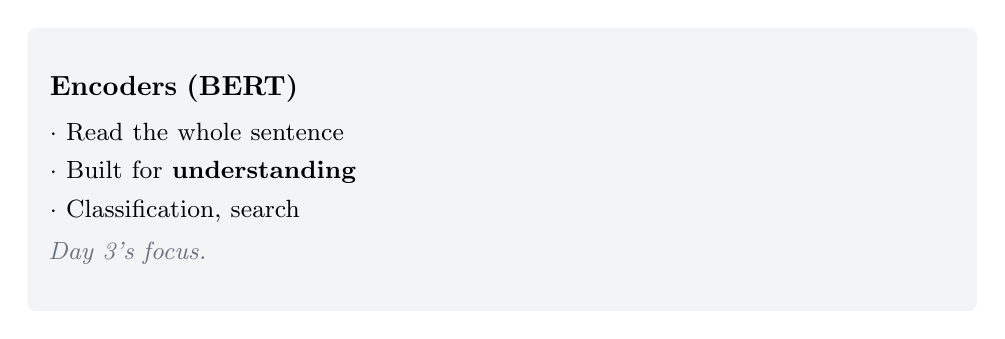
\begin{tikzpicture}
    \node[fill=lightgray, rounded corners=3pt,
          inner xsep=8pt, inner ysep=8pt, text width=\columnwidth-18pt, minimum height=3.6cm]{%
      \textbf{Encoders (BERT)}\\[5pt]
      {\small
      $\cdot$ Read the whole sentence\\[3pt]
      $\cdot$ Built for \textbf{understanding}\\[3pt]
      $\cdot$ Classification, search\\[3pt]
      \textcolor{midgray}{\textit{Day 3's focus.}}}};
  \end{tikzpicture}

  \column{0.48\textwidth}
  \vspace{0pt}
  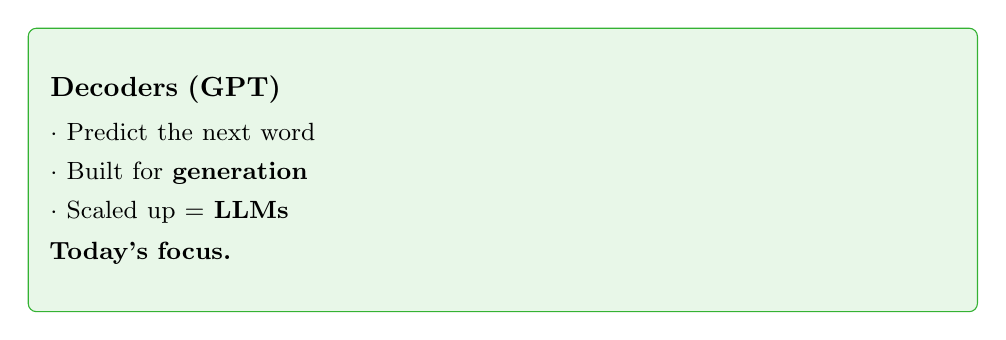
\begin{tikzpicture}
    \node[fill=lightgreen, draw=wurgreen, rounded corners=3pt,
          inner xsep=8pt, inner ysep=8pt, text width=\columnwidth-18pt, minimum height=3.6cm]{%
      \textbf{Decoders (GPT)}\\[5pt]
      {\small
      $\cdot$ Predict the next word\\[3pt]
      $\cdot$ Built for \textbf{generation}\\[3pt]
      $\cdot$ Scaled up = \textbf{LLMs}\\[3pt]
      \textbf{Today's focus.}}};
  \end{tikzpicture}
\end{columns}

\medskip
{\small\textcolor{midgray}{\textit{Take a decoder, make it enormous, train it on much of the
internet --- and you get a \textbf{Large Language Model}.}}}
\end{frame}

% ── SLIDE 2: next-token prediction ────────────────────────────────────────
\begin{frame}{What an LLM Actually Does: Predict the Next Word}
\vspace{0.2cm}
{\small At heart, an LLM does something almost absurdly simple: given some text, it predicts
\textbf{the most likely next word} --- over and over.}

\medskip
\begin{center}
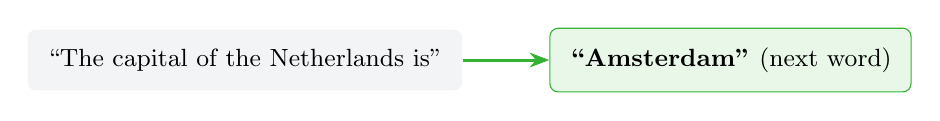
\begin{tikzpicture}[font=\small]
  \node[fill=lightgray, rounded corners=3pt, inner sep=7pt] (ctx)
    {``The capital of the Netherlands is''};
  \node[right=1.1cm of ctx, fill=lightgreen, draw=wurgreen, rounded corners=3pt, inner sep=7pt] (pred)
    {\textbf{``Amsterdam''} (next word)};
  \draw[-{Stealth[length=2.5mm]}, wurgreen, line width=1.1pt] (ctx) -- (pred);
\end{tikzpicture}
\end{center}

\medskip
{\small Then it \textbf{appends} that word and predicts again. Repeat, and coherent paragraphs
emerge --- one word at a time. That is all ``generation'' is.}

\medskip
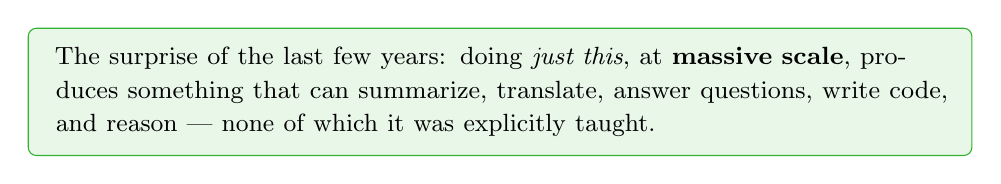
\begin{tikzpicture}
  \node[fill=lightgreen, draw=wurgreen, rounded corners=3pt,
        inner xsep=10pt, inner ysep=7pt, text width=\textwidth-24pt]{%
    {\small The surprise of the last few years: doing \emph{just this}, at \textbf{massive
    scale}, produces something that can summarize, translate, answer questions, write code,
    and reason --- none of which it was explicitly taught.}};
\end{tikzpicture}
\end{frame}

% ── SLIDE 3: scale ────────────────────────────────────────────────────────
\begin{frame}{The Magic Ingredient: Scale}
\vspace{0.2cm}
{\small Why is GPT-4 so different from the small models of a few years ago? Mostly
\textbf{scale} --- three things grew together, by orders of magnitude:}

\medskip
\begin{columns}[T]
  \column{0.31\textwidth}
  \vspace{0pt}
  \begin{tikzpicture}
    \node[fill=lightgray, rounded corners=3pt,
          inner xsep=7pt, inner ysep=8pt, text width=\columnwidth-16pt, minimum height=3.3cm]{%
      \textbf{\faDatabase\ Data}\\[5pt]
      {\small Much of the public internet --- \textbf{trillions} of words}};
  \end{tikzpicture}

  \column{0.31\textwidth}
  \vspace{0pt}
  \begin{tikzpicture}
    \node[fill=lightgray, rounded corners=3pt,
          inner xsep=7pt, inner ysep=8pt, text width=\columnwidth-16pt, minimum height=3.3cm]{%
      \textbf{\faProjectDiagram\ Parameters}\\[5pt]
      {\small From millions (BERT) to \textbf{hundreds of billions}}};
  \end{tikzpicture}

  \column{0.31\textwidth}
  \vspace{0pt}
  \begin{tikzpicture}
    \node[fill=lightgray, rounded corners=3pt,
          inner xsep=7pt, inner ysep=8pt, text width=\columnwidth-16pt, minimum height=3.3cm]{%
      \textbf{\faMicrochip\ Compute}\\[5pt]
      {\small Thousands of GPUs, months of training, huge cost}};
  \end{tikzpicture}
\end{columns}

\medskip
{\small As models grew, \textbf{new abilities appeared} that smaller models simply did not have
--- following instructions, few-shot learning, reasoning. This is why they are called
\emph{large} language models.}

\medskip
{\small\textcolor{midgray}{\textit{The flip side: that scale is expensive, concentrated in a few
companies, and has real costs --- we return to this in Part 2.}}}
\end{frame}

% ── SLIDE 4: instruction tuning / chat ────────────────────────────────────
\begin{frame}{From Word-Predictor to Assistant}
\vspace{0.2cm}
{\small A raw next-word predictor is not yet ChatGPT. Two extra steps turn it into a helpful
\textbf{assistant}:}

\medskip
\begin{columns}[T]
  \column{0.48\textwidth}
  \vspace{0pt}
  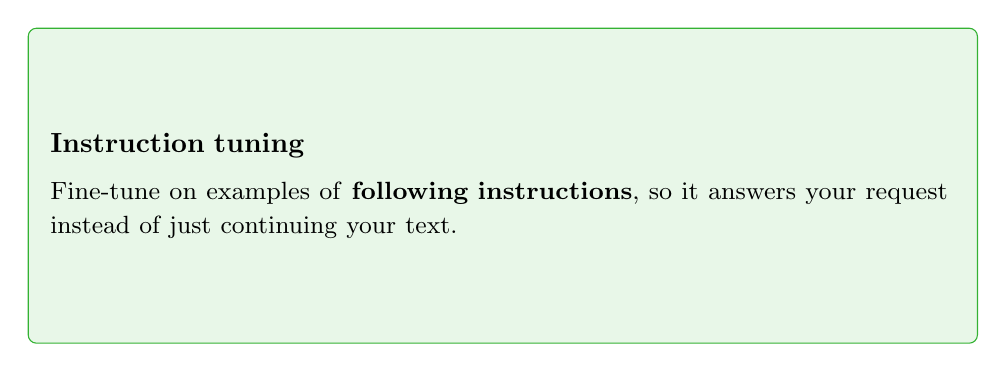
\begin{tikzpicture}
    \node[fill=lightgreen, draw=wurgreen, rounded corners=3pt,
          inner xsep=8pt, inner ysep=8pt, text width=\columnwidth-18pt, minimum height=4cm]{%
      \textbf{Instruction tuning}\\[5pt]
      {\small Fine-tune on examples of \textbf{following instructions}, so it answers your
      request instead of just continuing your text.}};
  \end{tikzpicture}

  \column{0.48\textwidth}
  \vspace{0pt}
  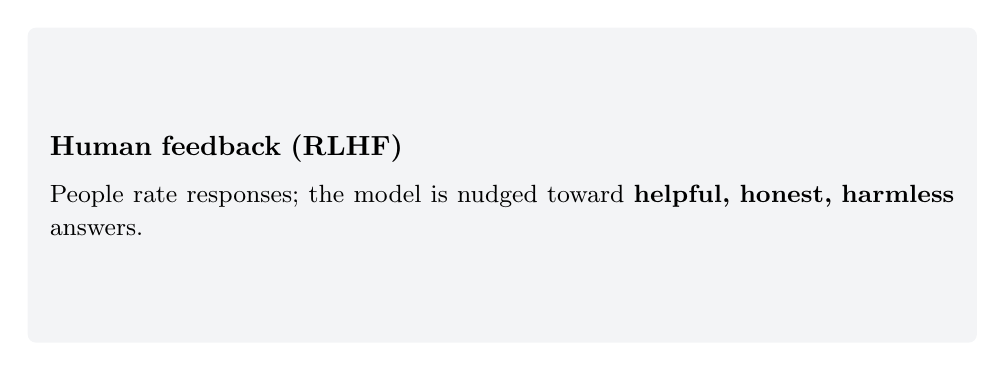
\begin{tikzpicture}
    \node[fill=lightgray, rounded corners=3pt,
          inner xsep=8pt, inner ysep=8pt, text width=\columnwidth-18pt, minimum height=4cm]{%
      \textbf{Human feedback (RLHF)}\\[5pt]
      {\small People rate responses; the model is nudged toward \textbf{helpful, honest,
      harmless} answers.}};
  \end{tikzpicture}
\end{columns}

\medskip
{\small\textcolor{midgray}{\textit{You mostly interact with instruction-tuned models --- but
under the hood, it is still next-word prediction.}}}
\end{frame}

% ── SLIDE 5: what can they be used for (overview) ─────────────────────────
\begin{frame}{What Can LLMs Do? A Sampler}
\vspace{0.2cm}
\begin{columns}[T]
  \column{0.48\textwidth}
  \vspace{0pt}
  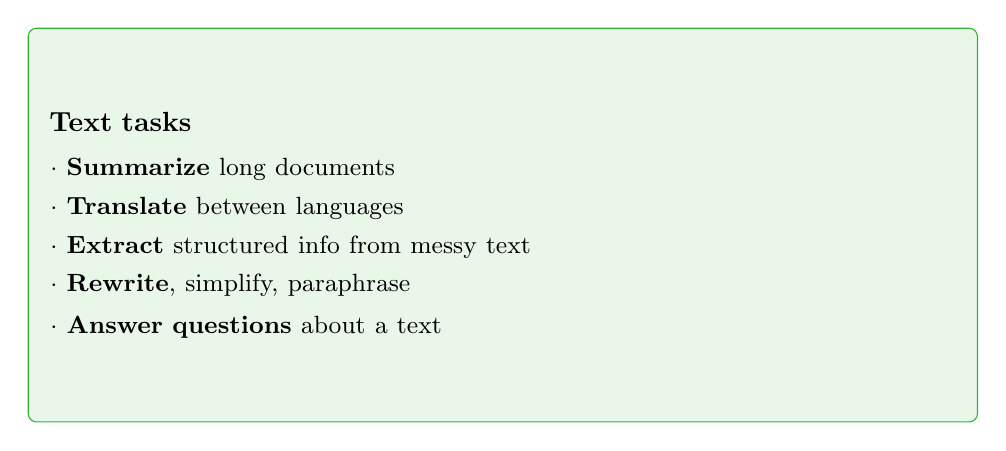
\begin{tikzpicture}
    \node[fill=lightgreen, draw=wurgreen, rounded corners=3pt,
          inner xsep=8pt, inner ysep=8pt, text width=\columnwidth-18pt, minimum height=5cm]{%
      \textbf{Text tasks}\\[5pt]
      {\small
      $\cdot$ \textbf{Summarize} long documents\\[3pt]
      $\cdot$ \textbf{Translate} between languages\\[3pt]
      $\cdot$ \textbf{Extract} structured info from messy text\\[3pt]
      $\cdot$ \textbf{Rewrite}, simplify, paraphrase\\[3pt]
      $\cdot$ \textbf{Answer questions} about a text}};
  \end{tikzpicture}

  \column{0.48\textwidth}
  \vspace{0pt}
  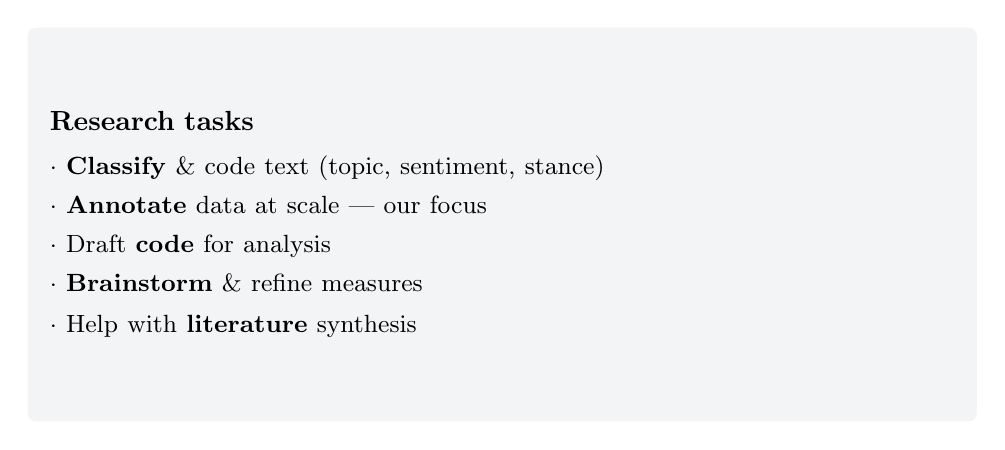
\begin{tikzpicture}
    \node[fill=lightgray, rounded corners=3pt,
          inner xsep=8pt, inner ysep=8pt, text width=\columnwidth-18pt, minimum height=5cm]{%
      \textbf{Research tasks}\\[5pt]
      {\small
      $\cdot$ \textbf{Classify} \& code text (topic, sentiment, stance)\\[3pt]
      $\cdot$ \textbf{Annotate} data at scale --- our focus\\[3pt]
      $\cdot$ Draft \textbf{code} for analysis\\[3pt]
      $\cdot$ \textbf{Brainstorm} \& refine measures\\[3pt]
      $\cdot$ Help with \textbf{literature} synthesis}};
  \end{tikzpicture}
\end{columns}

\medskip
{\small\textcolor{midgray}{\textit{A general-purpose text tool --- but ``general-purpose'' also
means ``not automatically reliable''. Every use needs validation.}}}
\end{frame}

% ── SLIDE 6: how you interact - prompting ─────────────────────────────────
\begin{frame}{How You Steer Them: Prompting}
\vspace{0.2cm}
{\small You control an LLM through the \textbf{prompt} --- the instructions and context you
give it. Three patterns you will use constantly:}

\medskip
\begin{columns}[T]
  \column{0.31\textwidth}
  \vspace{0pt}
  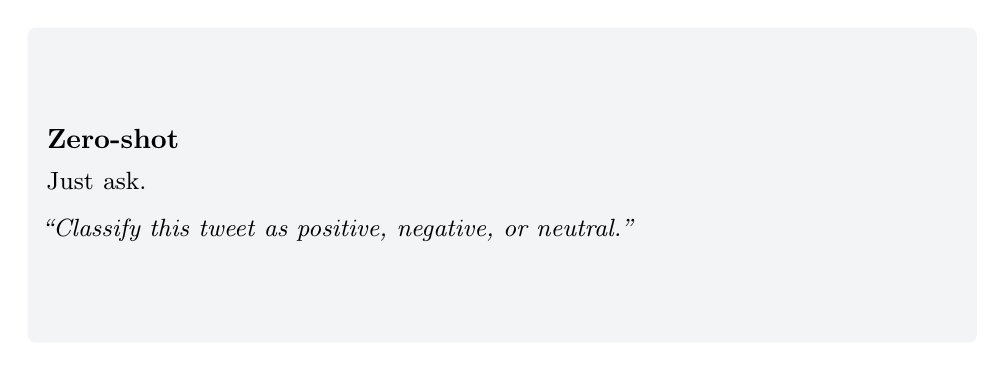
\begin{tikzpicture}
    \node[fill=lightgray, rounded corners=3pt,
          inner xsep=7pt, inner ysep=8pt, text width=\columnwidth-16pt, minimum height=4cm]{%
      \textbf{Zero-shot}\\[4pt]
      {\small Just ask.\\[5pt]
      \textit{``Classify this tweet as positive, negative, or neutral.''}}};
  \end{tikzpicture}

  \column{0.31\textwidth}
  \vspace{0pt}
  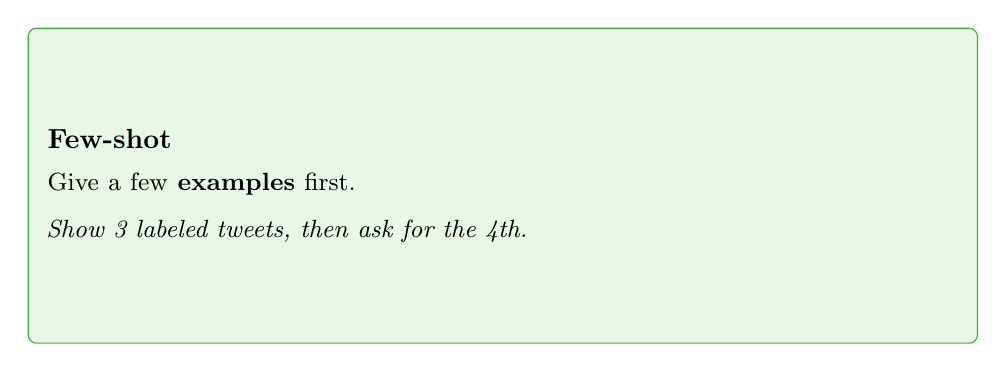
\begin{tikzpicture}
    \node[fill=lightgreen, draw=wurgreen, rounded corners=3pt,
          inner xsep=7pt, inner ysep=8pt, text width=\columnwidth-16pt, minimum height=4cm]{%
      \textbf{Few-shot}\\[4pt]
      {\small Give a few \textbf{examples} first.\\[5pt]
      \textit{Show 3 labeled tweets, then ask for the 4th.}}};
  \end{tikzpicture}

  \column{0.31\textwidth}
  \vspace{0pt}
  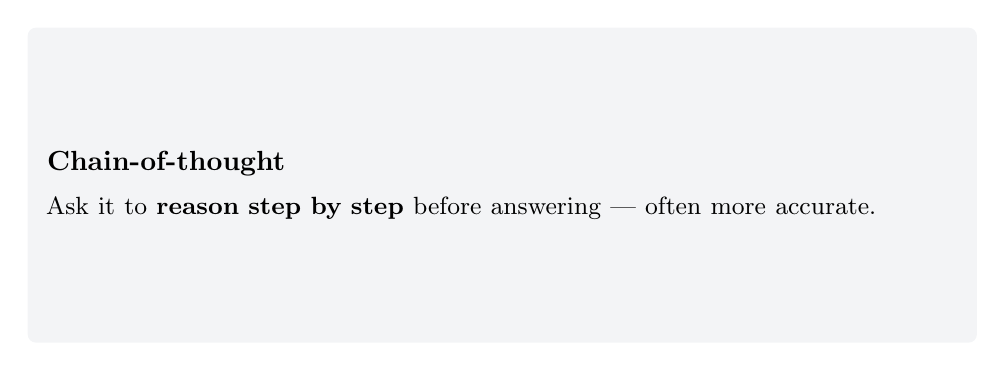
\begin{tikzpicture}
    \node[fill=lightgray, rounded corners=3pt,
          inner xsep=7pt, inner ysep=8pt, text width=\columnwidth-16pt, minimum height=4cm]{%
      \textbf{Chain-of-thought}\\[4pt]
      {\small Ask it to \textbf{reason step by step} before answering --- often more accurate.}};
  \end{tikzpicture}
\end{columns}

\medskip
{\small\textcolor{midgray}{\textit{Prompt wording matters a lot --- and that is both a strength
(flexible) and a weakness (fragile, hard to reproduce). More on this in Part 2.}}}
\end{frame}

% ── SLIDE 7: annotation - the big use case ────────────────────────────────
\begin{frame}{The Use Case We Care About: Data Annotation}
\vspace{0.2cm}
{\small For social scientists, one LLM use stands out: \textbf{annotating (coding) text data}.
Traditionally this means armies of human coders. LLMs can do a lot of it --- fast and cheap.}

\medskip
\begin{center}
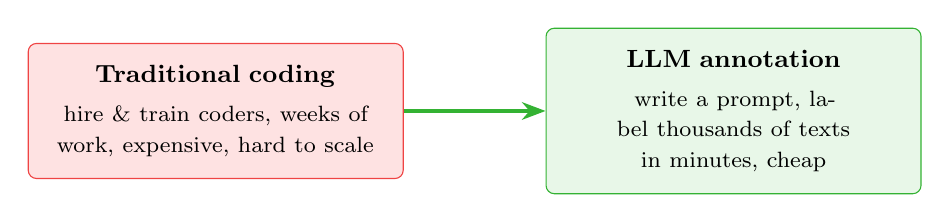
\begin{tikzpicture}[font=\small, node distance=0.9cm]
  \node[fill=warnred, draw=warnborder, rounded corners=3pt, inner sep=8pt, text width=4.2cm, align=center] (old)
    {\textbf{Traditional coding}\\[3pt]{\footnotesize hire \& train coders, weeks of work, expensive, hard to scale}};
  \node[fill=lightgreen, draw=wurgreen, rounded corners=3pt, inner sep=8pt,
        text width=4.2cm, align=center, right=1.8cm of old] (new)
    {\textbf{LLM annotation}\\[3pt]{\footnotesize write a prompt, label thousands of texts in minutes, cheap}};
  \draw[-{Stealth[length=3mm]}, wurgreen, line width=1.2pt] (old) -- (new);
\end{tikzpicture}
\end{center}

\medskip
{\small Give the model your \textbf{codebook} as a prompt, feed it each text, and collect the
labels. Studies increasingly show LLMs can \textbf{match or approach human coders} on many
tasks --- at a fraction of the cost and time.}
\end{frame}

% ── SLIDE 8: annotation - how it works ────────────────────────────────────
\begin{frame}{How LLM Annotation Works in Practice}
\vspace{0.2cm}
{\small The recipe is simple. Turn your \textbf{codebook} into a prompt, loop over your texts,
parse the answers.}

\medskip
\begin{center}
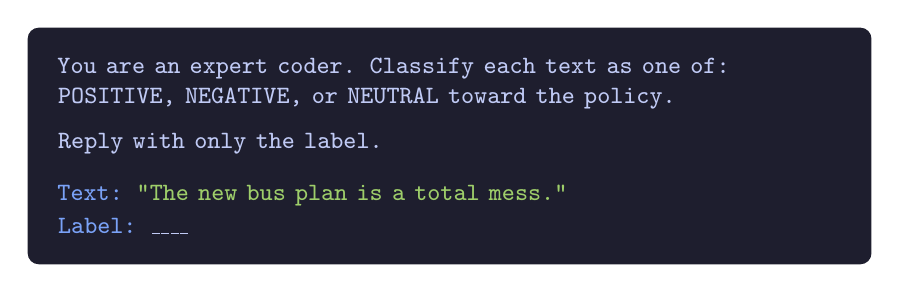
\begin{tikzpicture}
  \node[fill=codebg, rounded corners=4pt, inner sep=11pt, text width=0.82\textwidth, text=codegray]{%
    \ttfamily\small
    \textcolor{codegray}{You are an expert coder. Classify each text as one of:}\\
    \textcolor{codegreen}{}\textcolor{codegray}{POSITIVE, NEGATIVE, or NEUTRAL toward the policy.}\\[5pt]
    \textcolor{codegray}{Reply with only the label.}\\[8pt]
    \textcolor{codeblue}{Text:} \textcolor{codegreen}{"The new bus plan is a total mess."}\\
    \textcolor{codeblue}{Label:} \textcolor{codegray}{\_\_\_\_}%
  };
\end{tikzpicture}
\end{center}

\medskip
{\small The same prompt runs across your whole corpus. You can add your \textbf{definitions},
\textbf{examples} (few-shot), and \textbf{edge-case rules} --- exactly the things a human
codebook contains.}
\end{frame}

% ── SLIDE 9: annotation caveats ───────────────────────────────────────────
\begin{frame}{Annotation: Powerful, But Validate!}
\vspace{0.3cm}
\begin{columns}[T]
  \column{0.48\textwidth}
  \vspace{0pt}
  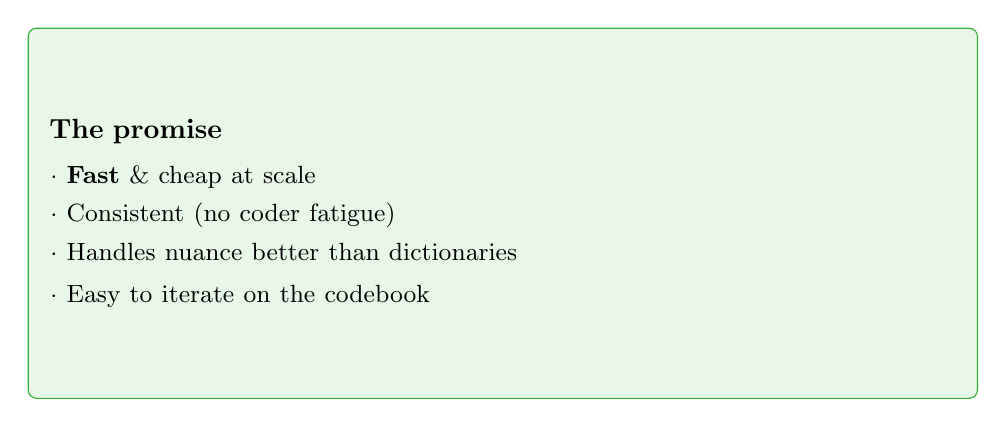
\begin{tikzpicture}
    \node[fill=lightgreen, draw=wurgreen, rounded corners=3pt,
          inner xsep=8pt, inner ysep=8pt, text width=\columnwidth-18pt, minimum height=4.7cm]{%
      \textbf{The promise}\\[5pt]
      {\small
      $\cdot$ \textbf{Fast} \& cheap at scale\\[3pt]
      $\cdot$ Consistent (no coder fatigue)\\[3pt]
      $\cdot$ Handles nuance better than dictionaries\\[3pt]
      $\cdot$ Easy to iterate on the codebook}};
  \end{tikzpicture}

  \column{0.48\textwidth}
  \vspace{0pt}
  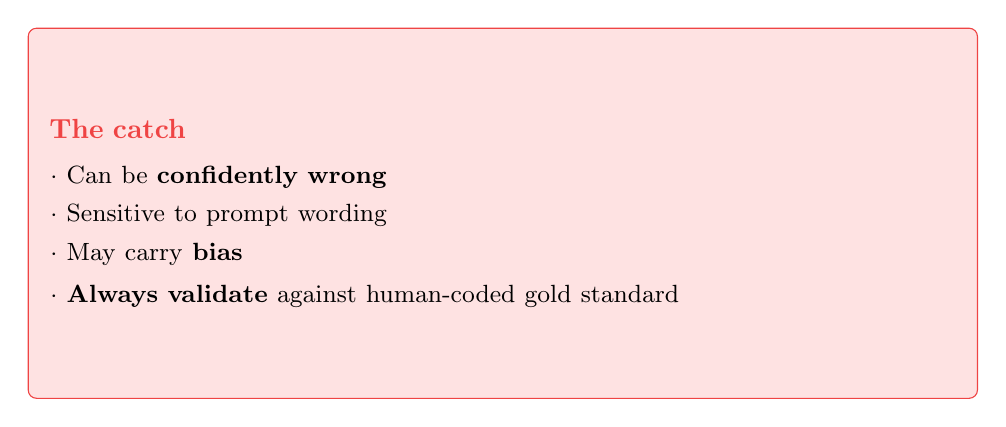
\begin{tikzpicture}
    \node[fill=warnred, draw=warnborder, rounded corners=3pt,
          inner xsep=8pt, inner ysep=8pt, text width=\columnwidth-18pt, minimum height=4.7cm]{%
      \textcolor{warnborder}{\textbf{The catch}}\\[5pt]
      {\small
      $\cdot$ Can be \textbf{confidently wrong}\\[3pt]
      $\cdot$ Sensitive to prompt wording\\[3pt]
      $\cdot$ May carry \textbf{bias}\\[3pt]
      $\cdot$ \textbf{Always validate} against human-coded gold standard}};
  \end{tikzpicture}
\end{columns}

\medskip
{\small\textcolor{midgray}{\textit{The golden rule: hand-code a sample yourself, measure
agreement with the LLM, and report it. An LLM annotator is a \textbf{measurement instrument} ---
and instruments must be validated.}}}
\end{frame}

% ── SLIDE 10: recap ───────────────────────────────────────────────────────
\begin{frame}{Part 1: The Takeaways}
\vspace{0.25cm}
\begin{itemize}\setlength\itemsep{7pt}
  \item[\textcolor{wurgreen}{\faCheck}]
    An \textbf{LLM} is a scaled-up decoder transformer that \textbf{predicts the next word}
  \item[\textcolor{wurgreen}{\faCheck}]
    \textbf{Scale} (data, parameters, compute) is what unlocked their surprising abilities
  \item[\textcolor{wurgreen}{\faCheck}]
    They are \textbf{general-purpose text tools} --- summarize, translate, classify, and more
  \item[\textcolor{wurgreen}{\faCheck}]
    You steer them by \textbf{prompting} (zero-shot, few-shot, chain-of-thought)
  \item[\textcolor{wurgreen}{\faCheck}]
    For research, \textbf{data annotation} is the killer app --- but \textbf{always validate}
    against human coders
\end{itemize}

\medskip
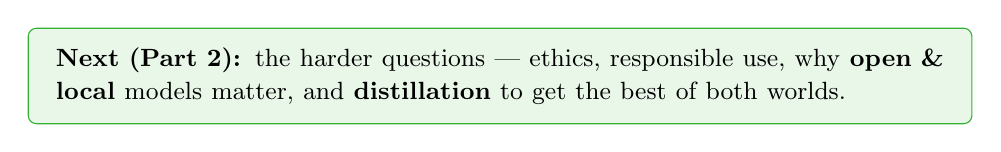
\begin{tikzpicture}
  \node[fill=lightgreen, draw=wurgreen, rounded corners=3pt,
        inner xsep=10pt, inner ysep=7pt, text width=\textwidth-24pt]{%
    {\small \textbf{Next (Part 2):} the harder questions --- ethics, responsible use, why
    \textbf{open \& local} models matter, and \textbf{distillation} to get the best of both
    worlds.}};
\end{tikzpicture}
\end{frame}

\end{document}
